
\begin{appendices}

\chapter{IQ Demodulation}\label{apx:iq}

\gls{iq} demodulation involves the process of transforming a signal on form 
\begin{equation}\label{eq:signal}
	x(t)=A(t)\sin(f_c t+\phi(t))
\end{equation}
to complex form without the carrier frequency $f_c$ \citep{lee_1991}
\begin{equation}
	x_{IQ}(t) = A(t)e^{i\phi(t)}.
\end{equation}
	
IQ demodulation thus aims to extract the information bearing part of $x(t)$ found in the envelope $A(t)$ and phase shift $\phi(t)$ from \eqref{eq:signal}. Most classical radars follow the demodulation scheme depicted in figure \ref{fig:iq_demod}. The first step is to split the signal in \eqref{eq:signal} into two separate channels. In the upper channel, the signal is multiplied by a coherent sinusoid with the same carrier frequency as the received pulse. The result of this multiplication can be rewritten as
\begin{equation}
	 A(t)\sin(f_c t+\phi(t))\cdot 2\sin(f_c t) = \\
\end{equation}
\begin{equation}\label{eq:split}
	A(t)\cos(\phi(t))-A(t)\cos(2f_c t+\phi(t))
\end{equation}
yielding one baseband sinusoid and one sinusoid at the double carrier frequency. 

The next step in the demodulation scheme is to low pass filter to get rid of the undesired high frequency term term in \eqref{eq:split} leaving only $A(t)\cos(\phi(t))$. This constitutes the \emph{In-phase} channel $I(t)$.

	Similarly, in the bottom channel in figure \ref{fig:iq_demod}, $x(t)$ is multiplied by a signal of the same carrier frequency. However, this time, the signal is shifted $90^\circ$ in phase\footnote{This shift is technically a \emph{Hilbert transform}, as the sinusoid is shifted by $\pi/2$.}. We can rewrite this product as
\begin{equation}
	 A(t)\sin(f_c t+\phi(t))\cdot 2\cos(f_c t) = 
\end{equation}
\begin{equation}\label{eq:split2}
 	 A(t)\sin(\phi(t))+A(t)\sin(2f_c t+\phi(t)).
\end{equation}

After low pass filtering we obtain $A(t)\sin(\phi(t))$ which we define as the \emph{Quadrature} channel $Q(t)$. Finally, by interpreting $I(t)$ and $Q(t)$ channels as the real- and imaginary parts of a complex number, respectively, we obtain our \gls{iq} data as
\begin{equation}
	I(t)+iQ(t)=A(t)\Big(\cos(\phi(t))+i\sin(\phi(t))\Big)=A(t)e^{i\phi(t)}.
\end{equation}

\begin{figure}
	\centering
	\hbox{\hspace{-0.5em} 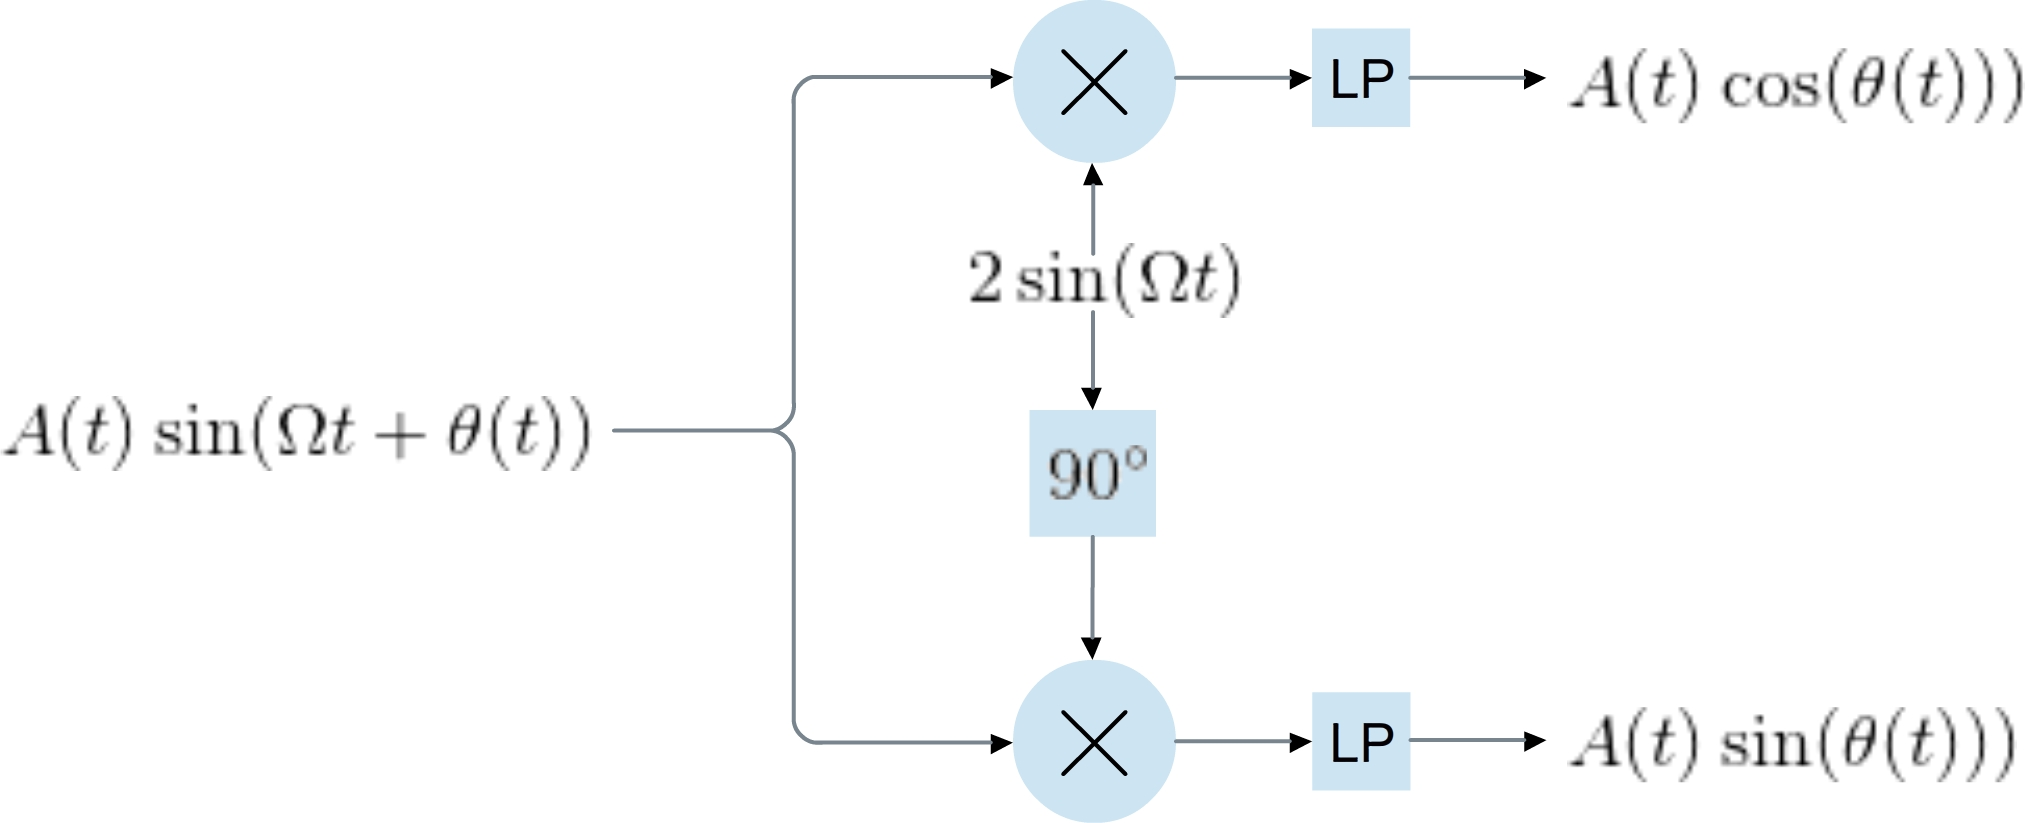
\includegraphics[scale=0.60]{figs_temp/iq_demod.jpg}}
	\caption{Schematics for a typical IQ demodulation.}
	\label{fig:iq_demod}
\end{figure}

% ######### MIXING PROOF ##########
\chapter{Proof of 2.15, 2.16 and 2.17}\label{apx:conv}

For signals $y(t)$ and $x_T(t)$ defined as
\begin{equation}
	\begin{split}
		y(t) &= CA(t - B)\sin(\Omega(t - B)) \\
		x_T(t) &= A(t)\sin(\Omega t) \\
	\end{split}
\end{equation}
with angular carrier frequency $\Omega = 2\pi f_c$, where $A(t)$ is defined as 
\begin{equation}
	A(t) = \begin{cases}
		1 & \text{if $0 \leq t < L$} \\
		0 & \text{otherwise}
	\end{cases}
\end{equation}
the output $m(\tau)$ of the matched filtering process becomes
\begin{equation}
	m(\tau) 
	= \int_{-\infty}^{+\infty}y(t)x_T(t-\tau)dt
\end{equation}
\begin{equation}	
	= C \int_{-\infty}^{+\infty}A(t-B)A(t-\tau)\sin(\Omega(t-B))\sin(\Omega(t-\tau))dt.
\end{equation}

This integral can be split into three cases:
\begin{enumerate}[label=(\roman*)]
	\item When $|\tau-B| \geq L$, i.e. when no overlap occurrs. 
	\item When $|\tau-B| < L$ and $\tau \leq B$.
	\item When $|\tau-B| < L$ and $\tau > B$.
\end{enumerate}

The first case, (i), clearly results in the integral becoming 0. Case (ii) can be written as
\begin{equation}
	m(\tau)
	= C\int_{B}^{\tau+L}\sin(\Omega(t-B))\sin(\Omega(t-\tau))dt
\end{equation}
\begin{equation}
	= \frac{C}{2}\int_B^{\tau+L} \cos(\Omega(\tau-B)) - \cos(\Omega(2t - B - \tau))dt
\end{equation}
\begin{equation}
	= \frac{C}{2}\Big( (\tau+L-B)\cos(\Omega(B-\tau)) 
	- \frac{1}{2\Omega}\Big[ \sin(\Omega(2t-B-\tau) \Big]_{B}^{\tau+L} \Big)
\end{equation}
\begin{equation}\label{eq:long}
	= \frac{C}{2}\Big((\tau + L - B)\cos(\Omega(B-\tau))
	- \frac{1}{2\Omega}\big(
	\sin(\Omega(\tau + 2L - B))
	- \sin(\Omega(B-\tau))
	\big)\Big)
\end{equation}

Selecting $L$ as a whole number $n$ of wavelengths $\lambda$, the argument of the second sinusoid can be simplified into
\begin{equation}
	\Omega(\tau + 2L - B) 
	= \Omega(\tau - B) + 2\frac{2\pi f n\lambda}{c} 
\end{equation}
\begin{equation}
	= \Omega(\tau - B) + 2\frac{2\pi f n c}{c f}
	= \Omega(\tau - B) + 4\pi n.
\end{equation}

This means that, as the sinus function is odd and $2\pi$ periodic, \eqref{eq:long} can be rewritten as 
\begin{equation}\label{eq:first}
	 \frac{C}{2}\Big( (\tau+L-B)\cos(\Omega(\tau - B)) 
	- \frac{1}{\Omega}\sin(\Omega(\tau - B))\Big).
\end{equation}

For (iii), we get a similar integral differing in the integral limits

\begin{equation}
	m(\tau) 
	= \int_\tau^{B+L}\sin(\Omega(t-B))\sin(\Omega(t-\tau))dt
\end{equation}
which is calculated similarly to (ii) to yield

\begin{equation}\label{eq:latter}
	\frac{C}{2}\Big( (B + L - \tau)\cos(\Omega(\tau - B))
	+ \frac{1}{\Omega}\sin(\Omega(\tau - B))\Big).
\end{equation}

Thus, the full mixing output can be written as

\begin{equation}
	m(\tau) = \begin{cases}
		0 & \text{if $|\tau-B|\geq L$} \\
		\text{(\ref{eq:first})} & \text{if $|\tau-B| < L$ and $\tau \leq B$} \\
		\text{(\ref{eq:latter})} & \text{if $|\tau-B| < L$ and $\tau>B$}.
	\end{cases}
\end{equation}

\end{appendices}


